\subsection{SACRAMENTO model (model ID: 33)}
The SACRAMENTO model (fig.~\ref{fig:33_schematic}) is part of an ongoing model development project by the National Weather Service, which started several decades ago \citep{Burnash1995,NationalWeatherService2005}. The documentation mentions a specific order of flux computations. For consistency with other models, here all fluxes are computed simultaneously. It has 5 stores and 13 parameters ($PCTIM$, $UZTWM$, $UZFWM$, $k_{uz}$, $PBASE$, $ZPERC$, $REXP$, $LZTWM$, $LZFWPM$, $LZFWSM$, $PFREE$, $k_{lzp}$ and $k_{lzs}$). The model also uses several coefficients derived from the calibration parameters \citep{Koren2000}: $PBASE$ and $ZPERC$. The model aims to represent:

\begin{itemizecompact}
\item Impervious and direct runoff;
\item Within soil division of water storage between tension and free water;
\item Surface runoff, interflow and percolation to deeper soil layers;
\item Multiple baseflow processes.
\end{itemizecompact}

\subsubsection{File names}
\begin{tabular}{@{}ll}
Model: &m\_33\_sacramento\_11p\_5s \\
Parameter ranges: &m\_33\_sacramento\_11p\_5s\_parameter\_ ranges \\
\end{tabular}

% Equations
\subsubsection{Model equations}

% Model layout figure
{ 																	% This ensures it doesn't warp text further down
\begin{wrapfigure}{l}{6cm}
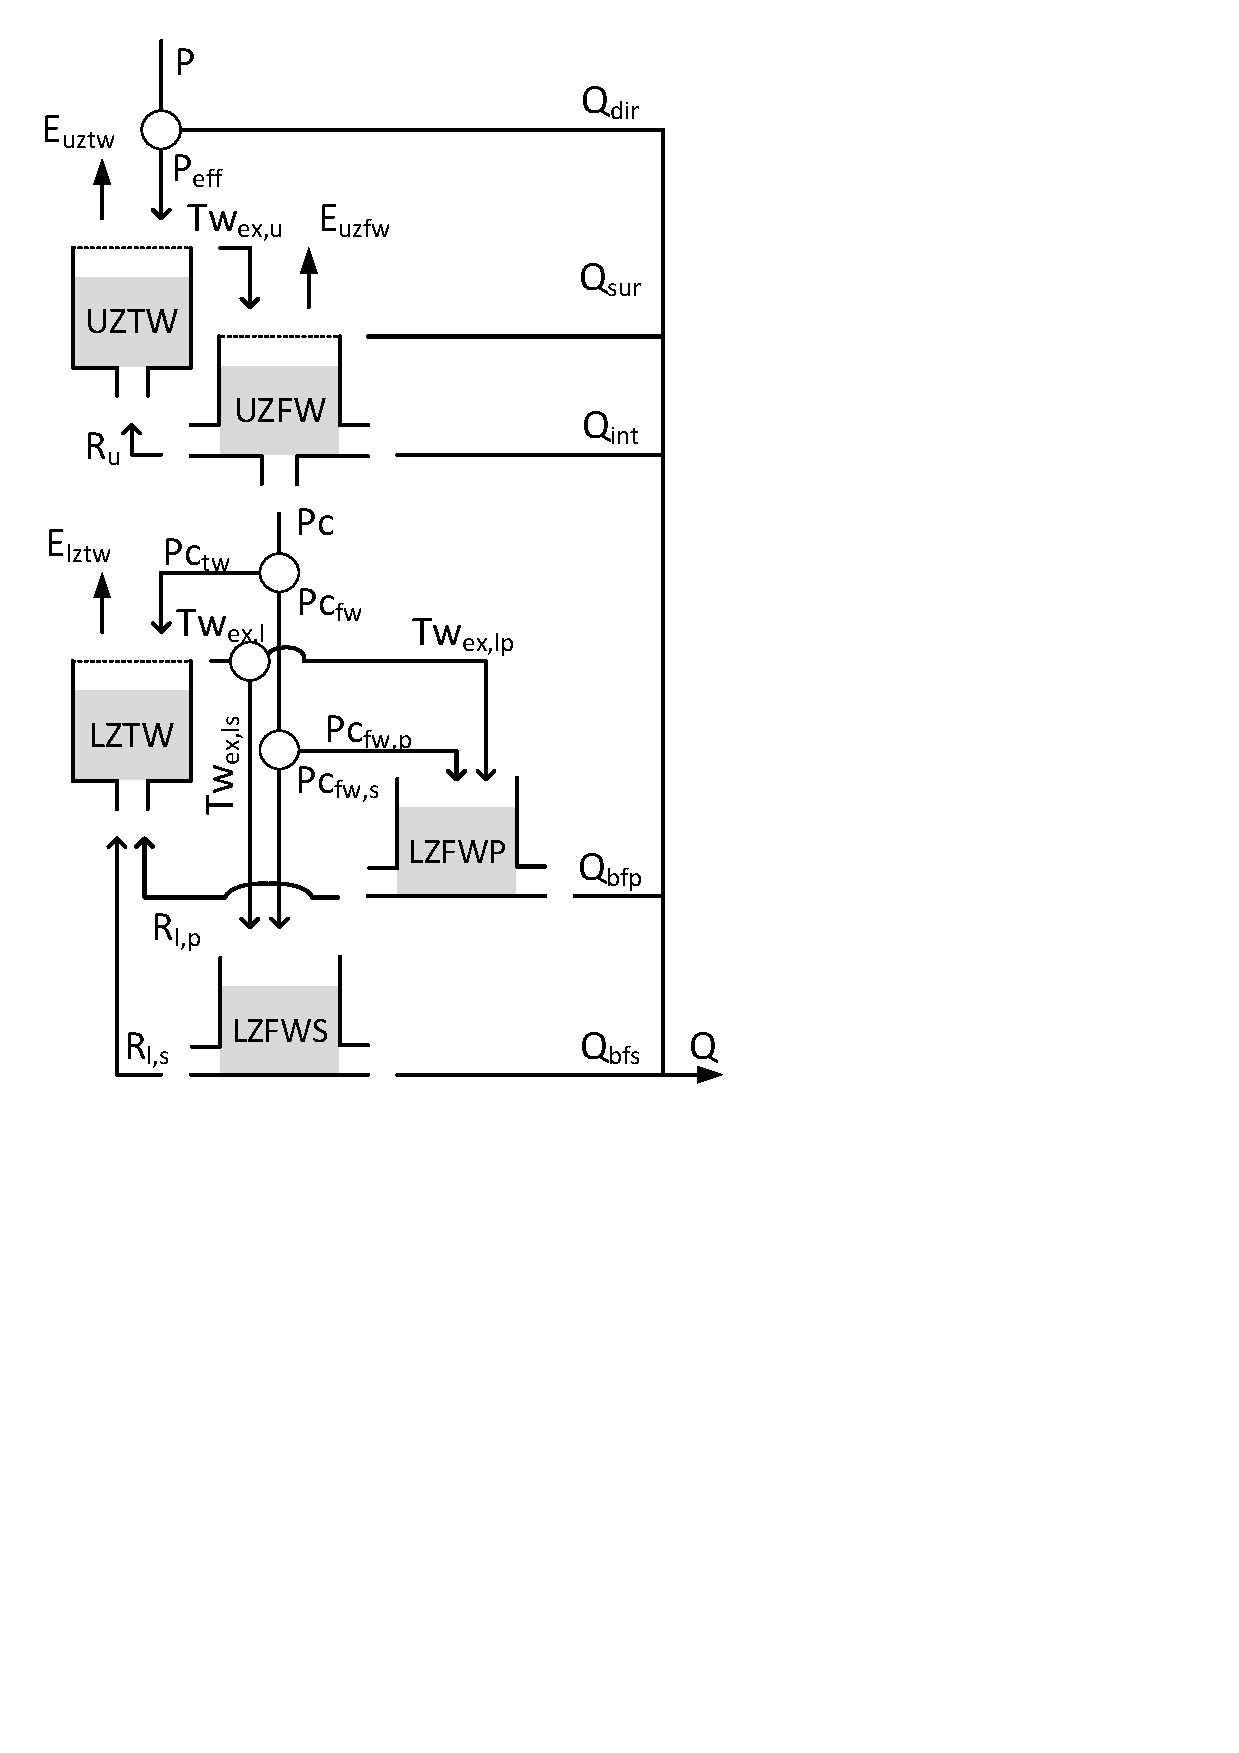
\includegraphics[trim=1cm 11cm 7cm 1cm,width=7cm,keepaspectratio]{./files/33_schematic.pdf}
\caption{Structure of the SACRAMENTO model} \label{fig:33_schematic}
\end{wrapfigure}

\begin{align}
	\frac{dUZTW}{dt} &= P_{eff} + R_u -E_{uztw}-Tw_{ex,u} \\
	P_{eff} &= (1-PCTIM)*P\\
	Q_{dir} &= PCTIM*P\\
	R_u &= \begin{cases} 
		\begin{aligned}
			\frac{UZTWM*UZFW-UZFWM*UZTW}{UZTWM+UZFWM}, \\	
			\text{if } \frac{UZTW}{UZTWM} < \frac{UZFW}{UZFWM} \\
		\end{aligned}\\
		0, \quad \text{otherwise} \\
	\end{cases}\\
	E_{uztw} &= \frac{UZTW}{UZTWM}*E_p\\
	Tw_{ex,u} &= \begin{cases}
		P_{eff}, &\text{if } UZTW = UZTWM \\
		0, & \text{otherwise} \\
	\end{cases} 
\end{align}

Where $UZTW$ [mm] is upper zone tension water, refilled by effective precipitation 

} % end of wrapfigure fix

\noindent$P_{eff}$ $[mm/d]$ and redistribution of free water $R_u$  $[mm/d]$, and is drained by evaporation $E_{uztw}$ $[mm/d]$ and tension water excess $Tw_{ex,u}$ $[mm/d]$.
$P_{eff}$ is the fraction $(1-PCTIM)$ [-] of precipitation $P$ that does not fall on impervious fraction $PCTIM$ [-].
$Q_{dir}$ $[mm/d]$ is the corresponding fraction direct runoff.
$R_u$ is only active when the relative deficit in tension water is greater than that in free water, and rebalances the available water in the upper zone. This uses the current storages, $UZTW$ and $UZFW$, and maximum storages, $UZTWM$ [mm] and $UZFWM$ [mm], of tension and free water stores respectively.
Evaporation is determined with a linear relation between available, maximum upper zone tension storage and potential evapotranspiration $E_p$ [mm/d].
$Tw_{ex,u}$ occurs only when the store is at maximum capacity.



\begin{align}
	\frac{dUZFW}{dt} &= Tw_{ex,u} - E_{uzfw} - Q_{sur} - Q_{int} - Pc - R_u \\
	E_{uzfw} &= \begin{cases}
		E_p-E_{uztw}, &\text{if } UZFW > 0 ~\&~ E_p>E_{uztw} \\
		0, & \text{otherwise} \\
	\end{cases}\\
	Q_{sur} &= \begin{cases}
		Tw_{ex,u}, &\text{if } UZFW = UZFWM \\
		0, & \text{otherwise} \\
	\end{cases}\\
	Q_{int} &= k_{uz} * UZFW\\
	Pc &= Pc_{demand} *\frac{UZFW}{UZFWM}\\
	Pc_{demand} &= PBASE*\left(1+ZPERC*\left(\frac{\sum{LZ_{deficiency}}}{\sum{LZ_{capacity}}}\right)^{1+REXP}\right)\\
	LZ_{deficiency} &= [LZTWM-LZTW]+[LZFWPM-LZWFP]+[LZFWSM-LZFWS]\\
	LZ_{capacity} &= LZTWM+LZFWPM+LZFWSM
\end{align}

Where $UZFW$ [mm] is upper zone free water, refilled by excess water $Tw_{ex,u}$ that can not be stored as tension water, and drained by evaporation  $E_{uzfw}$ $[mm/d]$, surface runoff $Q_{sur}$ $[mm/d]$, interflow $Q_{int}$ $[mm/d]$, and percolation to deeper groundwater $Pc$ $[mm/d]$.
Evaporative demand unmet by the upper tension water store is taken from upper free water storage at the potential rate.
$Q_{sur}$ occurs only when the store is at maximum capacity $UZFWM$ [mm].
$Q_{int}$ uses time coefficient $k_{uz}$ $[d^{-1}]$ to simulate interflow.
Percolation $Pc$ is calculated as a balance between the fraction water availability in upper zone free storage, and demand from the lower zone $Pc_{demand}$. The demand can be between a base percolation rate $PBASE$ $[mm/d]$ and an upper limit of $ZPERC$ [-] times $PBASE$. This demand is scaled by the relative size of lower zone moisture deficiencies, expressed as the ratio between total deficiency and maximum lower zone storage. $LZTWM$ [mm], $LZFWP$ [mm], $LZFWS$ [mm] are the maximum capacity of the lower zone tension store, primary free water store and supplemental free water store respectively. The lower zone percolation demand is potentially non-linear through exponent $REGX$ [-]. $PBASE$ is calculated as $k_{lzp}*LZFWPM+K_{lzs}*LZFWSM$.

\begin{align}
	\frac{dLZTW}{dt} &= Pc_{tw} + R_{l,p} + R_{l,s} - E_{lztw} - Tw_{ex,l} \\
	Pc_{tw} &= (1-PFREE)*Pc\\
	R_{l,p} &= \begin{cases}
		\begin{aligned}
		LZFWPM*\frac{-LZTW(LZFWPM+LZFWSM)+LZTWM(LZWFP+LZWFS)}{(LZFWPM+LZFWSM)(LZTWM+LZFWPM+LZFWSM)}, \\
				\text{if } \frac{LZTW}{LZTWM} < \frac{LZFWP+LZFWS}{LZFWPM+LZFWSM}\\
		\end{aligned}\\
		0, \quad \text{otherwise} \\
	\end{cases}\\	
	R_{l,s} &= \begin{cases}
		\begin{aligned}
		LZFWSM*\frac{-LZTW(LZFWPM+LZFWSM)+LZTWM(LZWFP+LZWFS)}{(LZFWPM+LZFWSM)(LZTWM+LZFWPM+LZFWSM)}, \\
			\text{if } \frac{LZTW}{LZTWM} < \frac{LZFWP+LZFWS}{LZFWPM+LZFWSM}\\
		\end{aligned}\\
		0, \quad \text{otherwise} \\
	\end{cases}\\	
	E_{lztw} &= \begin{cases}
		\left(E_p-E_{uztw}-E_{uzfw}\right)*\frac{LZTW}{UZTWM+LZTWM}, &\text{if } LZTW > 0 ~\&~ E_p > (E_{uztw}+E_{uzfw}) \\
		0, & \text{otherwise} \\
	\end{cases}\\
	Tw_{ex,l} &= \begin{cases}
		Pc_{tw}, &\text{if } LZTW = LZTWM \\
		0, & \text{otherwise} \\
	\end{cases}
\end{align}

Where $ LZTW$ [mm] is lower zone tension water, refilled by percolation $Pc_{tw}$ $[mm/d]$ and drained by evaporation $E_{lztw}$ $[mm/d]$ and tension water excess $Tw_{ex,l}$ $[mm/d]$.
Evaporative demand unmet b the upper zone can be satisfied from the lower zone tension water store, scaled by the current lower zone storage relative to total tension zone storage.
Both $R_{l,p}$ and $R_{l,s}$ are only active when the relative deficit in tension water is greater than that in free water, and rebalances the available water in the lower zone. This uses the current storages, $LZTW$, $LZFWP$ and $LZFWS$, and maximum storages, $LZTWM$ [mm], $LZFWPM$ [mm] and $LZFWSM$ [mm], of the tension and free water stores respectively.
$Pc_{tw}$ is the fraction $(1-PFREE)$ [-] of percolation $Pc$ that does not go into free storage.
$Tw_{ex,l}$ occurs only when the store is at maximum capacity $LZTWM$ [mm].

\begin{align}
	\frac{dLZFWP}{dt} &= Pc_{fw,p} + Tw_{ex,lp} - Q_{bfp} \\
	Pc_{fw,p} &= \left[\frac{LZFWPM-LZFWP}{LZFWPM\left(\frac{LZFWPM-LZFWP}{LZFWPM}+\frac{LZFWSM-LZFWS}{LZFWSM}\right)}\right]*\left(PFREE*Pc\right)\\
	Tw_{ex,lp} &= \left[\frac{LZFWPM-LZFWP}{LZFWPM\left(\frac{LZFWPM-LZFWP}{LZFWPM}+\frac{LZFWSM-LZFWS}{LZFWSM}\right)}\right]*Tw_{ex,l}\\
	Q_{bfp} &= k_{lzp}*LZFWP
\end{align}

Where $LZFWP$ [mm] is current storage in the primary lower zone free water store, refilled by excess tension water $TW_{ex,lp}$ $[mm/d]$ and percolation $Pc_{fw,p}$ $[mm/d]$ and drained by primary baseflow $Q_{bfp}$ $[mm/d]$.
Refilling of both lower zone free water stores (primary and supplemental) is divided between the two based on their relative, scaled moisture deficiency.
Percolation from the upper zone $Pc_{fw,p}$ is scaled according to the relative current moisture deficit $\frac{LZFWPM-LZFWP}{LZFWM}$ compared to the total relative deficit in the lower free water stores $\left(\frac{LZFWPM-LZFWP}{LZFWPM}+\frac{LZFWSM-LZFWS}{LZFWSM}\right)$.
$Tw_{ex,lp}$ is a similarly scaled part of $Tw_{ex,l}$.
$Q_{bfp}$ uses time parameter $K_{lzp}$ $[d^{-1}]$ to estimate primary baseflow.

\begin{align}
	\frac{dLZFWS}{dt} &= Pc_{fw,s} + Tw_{ex,ls} - Q_{bfs} \\
	Pc_{fw,s} &= \left[\frac{LZFWSM-LZFWS}{LZFWSM\left(\frac{LZFWPM-LZFWP}{LZFWPM}+\frac{LZFWSM-LZFWS}{LZFWSM}\right)}\right]*\left(PFREE*Pc\right)\\
	Tw_{ex,ls} &= \left[\frac{LZFWSM-LZFWS}{LZFWSM\left(\frac{LZFWPM-LZFWP}{LZFWPM}+\frac{LZFWSM-LZFWS}{LZFWSM}\right)}\right]*Tw_{ex,l}\\
	Q_{bfs} &= k_{lzs}*LZFWS
\end{align}

Where $LZFWS$ [mm] is current storage in the supplemental free water lower zone store, refilled by excess tension water $TW_{ex,ls}$ $[mm/d]$ and percolation $Pc_{fw,s}$ $[mm/d]$, and drained by supplemental baseflow $Q_{bfs}$ $[mm/d]$. 
$Pc_{fw,s}$ is determined based on relative deficits in the lower zone free stores, as is $Tw_{ex,ls}$.
$Q_{bfs}$ uses time parameter $K_{lzs}$ $[d^{-1}]$ to estimate supplementary baseflow. Total simulated outflow:

\begin{align}
	Q_t &= Q_{dir} + Q_{sur} + Q_{int} + Q_{bfp} + Q_{bfs}
\end{align}

\newpage
\subsubsection{Parameter overview}
% Table generated by Excel2LaTeX from sheet 'Sheet1'
\begin{table}[htbp]
  \centering
    \begin{tabular}{lll}
    \toprule
    Parameter & Unit  & Description \\
    \midrule
    $PCTIM$ & $-$   & Fraction impervious area \\
    $UZTWM$ & $mm$  & Maximum upper zone tension water storage \\
    $UZFWM$ & $mm$  & Maximum upper zone free water storage \\
    $k_{uz}$ & $d^{-1}$ & Runoff coefficient \\
    $PBASE$ & $mm~d^{-1}$ & Base percolation rate \\
    $ZPERC$ & $-$   & Maximum percolation rate as multiple of $ZPERC$ \\
    $REXP$ & $-$   & Percolation non-linearity parameter \\
    $LZTWM$ & $mm$  & Maximum lower zone tension water storage \\
    $LZFWPM$ & $mm$  & Maximum lower zone primary free water storage \\
    $LZFWSM$ & $mm$  & Maximum lower zone secondary free water storage \\
    $PFREE$ & $-$   & Fraction of percolation to free storage \\
    $k_{lzp}$ & $d^{-1}$ & Runoff coefficient \\
    $k_{lzs}$ & $d^{-1}$ & Runoff coefficient \\
    \bottomrule
    \end{tabular}%
  \label{tab:addlabel}%
\end{table}%

